\documentclass[11pt]{article}

\usepackage{amsmath,mathtools,siunitx,amssymb}
\usepackage[a4paper,left=1.5cm,right=1.5cm,top=2cm,bottom=2cm]{geometry}
\usepackage{float,subcaption,graphicx}
\usepackage{enumitem,pifont}
\renewcommand{\labelitemi}{\ding{228}}
\renewcommand{\labelitemii}{\ding{229}}
\renewcommand{\labelitemiii}{\ding{225}}
\setlist[itemize]{noitemsep}
\usepackage[dvipsnames]{xcolor}
\usepackage{color,hyperref}
\hypersetup{colorlinks=true}

\newcommand{\tVVt}{\frac{|\tilde{V}_{ij}|^2}{|V_{ij}|^2}}
\newcommand{\tVV}{\frac{|\tilde{V}_{ij}|}{|V_{ij}|}}

\begin{document}
{\Large\bfseries CKM Modification for paper draft}
\section{CKM Measurement Overview}

\section{Basic Framework}
In the 2HDM, the Branching Ratio of a tree-level leptonic decay of a meson M can be written as
\begin{equation}
    \label{eq:brrh}
    \mathcal{B}r_{exp}[M\to l\nu_l] = \mathcal{B}r_{SM}[M\to l\nu_l]\times(1+r_H)^2.
\end{equation}
Here, $(1+r_H)^2$ describes the 2HDM correction factor, where for the meson M consisting of the up-type quark $q_u$ and down-type quark $q_d$,
\begin{equation}
    r_H = \left(\frac{m_{q_u}-m_{q_d}\tan^2\beta}{m_{q_u}+m_{q_d}}\right)\left(\frac{m_M}{m_{H^+}}\right)^2.
\end{equation}
This description of the 2HDM modification is convenient for working with leptonic decays, however when also considering semileptonic decays, $r_H$ can be broken down further into contributions to two Wilson coefficients for scalar operators defined as:
\begin{align}
    \mathcal{O}_{SR} = -\frac{4G_F}{\sqrt{2}}V_{ub}(\bar{u}_Lb_R)(\bar{\mu}_R\nu_{\mu L}) &\to C_{SR} = \frac{m_u}{m_{H^+}^2} \\
    \mathcal{O}_{SL} = -\frac{4G_F}{\sqrt{2}}V_{ub}(\bar{u}_Rb_L)(\bar{\mu}_L\nu_{\mu R}) &\to C_{SL} = \frac{m_b\tan^2\beta}{m_{H^+}^2} 
\end{align}
In Eq.\eqref{eq:brrh}, the CKM element $|V_{ij}|^2$ is included in $\mathcal{B}r_{SM}$, but if the 2HDM is realistic, then what we measure from experiment for the value of $|V_{ij}|^2$ is really $|V_{ij}|^2\times(1+r_H)^2$.\\
$r_H=0$ means that 2HDM is wrong, and we're back to the SM value being correct;
$r_H=-2$ means we're in the fine-tuned solution of the 2HDM and what we measure as the SM CKM element is the correct value, although the 2HDM is still correct;
$r_H\neq0,-2$ means that the real CKM element is different from the measured one and we can't use the given SM values.
So if we assume 2HDM to be right, we're probably using the wrong CKM element.
Now consider having
    \begin{equation*}
        \mathcal{B}r_{exp} = \mathcal{B}r_{SM}\times\tVVt(1+r_H)^2
    \end{equation*}
as our equation, with $\tilde{V}_{ij}$ being the `real' CKM element value and $V_{ij}$ being the measured one in the SM.
This lets us cancel the SM CKM value and input the `real' one, if there is a difference in their value.
For working in flavio, we need to write any modifications to SM formulae as NP WCs to be added to the SM WCs, so we need to rewrite this:
    \begin{align*}
        \tVVt(1+r_H)^2 &= \left\{\tVV+\tVV r_H\right\}^2 \\
                       &= \left\{1+\left(\tVV-1\right)+\tVV r_H\right\}^2
    \end{align*}
Writing like this means we can just add on $\tVV-1$ to a WC (e.g. to \textbf{CVL\_bumunumu} in \href{https://wcxf.github.io/assets/pdf/WET.flavio.pdf}{flavio's WET basis} for $B^+\to\mu^+\nu_\mu$) and just multiply the WCs involved with $r_H$ by $\tVV$.
If the CKM element is not changed in the 2HDM, its contribution to the above will go away and we'll be back to our original consideration for the 2HDM; if it is changed, then we will be able to notice it.
This leaves us with 3 free parameters to fit, and I'm not sure if we can do that properly within flavio as it is, but it is simple enough to build up a picture of this modification's impact by doing a range of 2D contours as before for various values of $\tVV$.
The issue with this is that then you have to fit for each quark current so that you're only considering a single CKM element at once, and for some, i.e. kaons and pions, their errors in form factors are quite large so I'm not sure if we can really resolve much information from those fits.\\
I've done some quick contours for various values of $\tVV$ for the leptonic decays we've been using, which you can look through at \href{https://github.com/mbr-phys/higgs-proj/tree/master/ckm_tests}{github/mbr-phys/higgs-proj/tree/master/ckm\_tests} in individual folders for each CKM element consider.\\
It would probably be worthwhile adding more leptonic decays to these fits for better indication of our validity of choice in $\tVV$ but I haven't looked into any extras yet.
Using our leptonic decays so far, we can analyse how Vud, Vus, Vub, Vcd, and Vcs can be modified in the 2HDM, but for the other elements, we would have to extract from unitarity.
We have all the first row elements here which means we could use unitarity as an extra constraint and test the elements together.
It might be possible to do similar to above for $\mathcal{R}(D^{(*)})$ and Vcb so we could then use unitarity constraints on the first two rows.\\
Since $\gamma$ comes from the phase of the elements, it shouldn't be affected by the 2HDM, so while just considering 2HDM, we can use the usual method to construct the full matrix from knowing how to modify Vub, Vcb, Vus.

\section{Mapping Out the Modification}
For leptonic decays, using $r_H$ as above, I've done some heatmaps showing values that $\tVV$ can take.
As James discussed in his notes, if the 2HDM is real then the value we measure and assume in the SM is
\begin{align*}
|V_{ij}|^2 = |\tilde{V}_{ij}|^2(1+r_H)^2 \implies \frac{1}{(1+r_H)} = \tVV.
\end{align*}
Again, all plots and code are on the github link if you want to look closer.
For each point in parameter space, I have taken the modification factors for each CKM element from the heatmaps, modified the accepted CKM elements accordingly, and tested for unitarity in the first two rows -- this is just using a scan, no statistics yet.
This is using purely leptonic modifications for the first five elements, and semileptonic modifications for $V_{cb}$ from the same principles:
\begin{figure}[H]
    \centering
    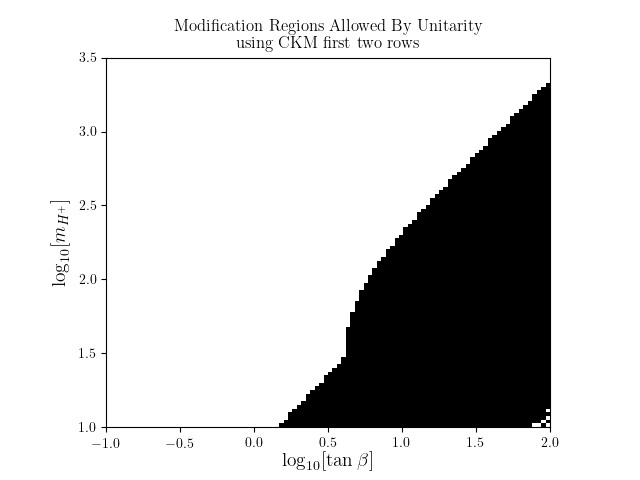
\includegraphics[width=0.45\textwidth]{heatmaps/mod.png}
    \caption{The black region represents areas where the first two rows of the CKM matrix break unitarity from 2HDM modification as discussed above; the white is where unitarity is still possible within $2\sigma$.}
\end{figure}

\section{Conclusions}
It looks like from my heatmaps and the unitarity scan that it is a reasonable assumption to neglect any modification to the CKM elements in the first two rows.
Direct searches limit $m_{H^+}\gtrsim160\,$GeV which cuts off most of the disallowed region in Figure 1.
Similarly, $b\to s\gamma$ will cut off practically all of the disallowed region -- I don't think that any minor modification of CKM elements will change $b\to s\gamma$ significantly so it should roughly remain the same as we've had previously, although it will be worth double checking this in case there is some additional effect.
From my heatmaps, we can see that there will be small modifications to some CKM elements, although these can be mostly negligible in the regions our fits are moving towards.\\ 
Instead of calculating for the CKM elements individually as I've done so far, I think what will be best moving forward is considering $|V_{ub}|,V_{us},V_{cb},\gamma$ only and checking unitarity and magnitudes of modifications of the full CKM matrix from the standard parameterisation calculation.
I have the framework from what I have done above for $|V_{ub}|,V_{us},V_{cb}$, so I need to work on modifications to $\gamma$ before I can give further results.
It is likely that there will not be much difference compared to the above results, but it is better to be rigorous in case there is.
From the definition of $\gamma$,
\begin{equation*}
    \gamma = \text{arg}\left(-\frac{V_{ud}V_{ub}^*}{V_{cd}V_{cb}^*}\right),
\end{equation*}
I would naively assume that the 2HDM will not modify it as it should only affect the CKM element magnitudes and not their complex phases.

\end{document}












